\section{Технологическая часть}

\subsection{Выбор языка и среды программирования}
В качестве языка программирования для выполнения поставленной
задачи был выбран язык С. Он является языком реализации большинства
модулей и драйверов ОС Linux. В качестве компилятора был использован
компилятор gcc. Средой разработки был выбран текстовый редактор
Visual Studio Code.

\subsection{Описание ключевых моментов реализации}
Основной структурой USB драйвера является \textit{struct usb\_driver}. Данная структура представлена в Листинге 1.

\begin{lstlisting}[caption=Структура usb\_driver]
	static struct usb_driver xpad_driver = {
		.name		= "myxpad",
		.probe		= xpad_probe,
		.disconnect	= xpad_disconnect,
		.id_table	= xpad_table,
	};
\end{lstlisting}

Локальной системной структурой является \textit{usb\_xpad}. Данная структура показана в Листинге 2.

\begin{lstlisting}[caption=Структура usb\_xpad]
	struct usb_xpad {
		struct input_dev *dev;		/* input device interface */
		struct usb_device *udev;	/* usb device */
		struct usb_interface *intf;	/* usb interface */
		
		int pad_present;
		
		struct urb *irq_in;		/* urb for interrupt in report */
		unsigned char *idata;		/* input data */
		dma_addr_t idata_dma;
		
		unsigned char *bdata;
		
		struct urb *irq_out;		/* urb for interrupt out report */
		unsigned char *odata;		/* output data */
		dma_addr_t odata_dma;
		struct mutex odata_mutex;
		
		char phys[64];			/* physical device path */
		
		int mapping;			/* map d-pad to buttons or to axes */
		int xtype;			/* type of xbox device */
	};
\end{lstlisting}

Ниже в Листинге 3 представлена функция инициализации при загрузке

драйвера \textit{xpad\_probe}.
\begin{lstlisting}[caption=Функция xpad\_probe]
	static int xpad_probe(struct usb_interface *intf, const struct usb_device_id *id)
	{
		printk("My XPAD is Connected");
		
		struct usb_device *udev = interface_to_usbdev(intf);
		struct usb_xpad *xpad;
		struct input_dev *input_dev;
		struct usb_endpoint_descriptor *ep_irq_in;
		int ep_irq_in_idx;
		int i, error;
		
		for (i = 0; xpad_device[i].idVendor; i++) {
			if ((le16_to_cpu(udev->descriptor.idVendor) == xpad_device[i].idVendor) &&
			(le16_to_cpu(udev->descriptor.idProduct) == xpad_device[i].idProduct))
			break;
		}
		
		xpad = kzalloc(sizeof(struct usb_xpad), GFP_KERNEL);
		input_dev = input_allocate_device();
		if (!xpad || !input_dev) {
			error = -ENOMEM;
			input_free_device(input_dev);
			kfree(xpad);
			return error;
		}
		
		xpad->idata = usb_alloc_coherent(udev, XPAD_PKT_LEN,
		GFP_KERNEL, &xpad->idata_dma);
		if (!xpad->idata) {
			error = -ENOMEM;
			input_free_device(input_dev);
			kfree(xpad);
			return error;
		}
		
		xpad->irq_in = usb_alloc_urb(0, GFP_KERNEL);
		if (!xpad->irq_in) {
			error = -ENOMEM;
			usb_free_coherent(udev, XPAD_PKT_LEN, xpad->idata, xpad->idata_dma);
			input_free_device(input_dev);
			kfree(xpad);
			return error;
		}
		
		xpad->udev = udev;
		xpad->intf = intf;
		xpad->mapping = xpad_device[i].mapping;
		xpad->xtype = xpad_device[i].xtype;
		
		if (xpad->xtype == XTYPE_UNKNOWN) {
			if (intf->cur_altsetting->desc.bInterfaceClass == USB_CLASS_VENDOR_SPEC) {
				if (intf->cur_altsetting->desc.bInterfaceProtocol == 129)
				xpad->xtype = XTYPE_XBOX360;
			} else
			xpad->xtype = XTYPE_XBOX;
			
			if (dpad_to_buttons)
			xpad->mapping |= MAP_DPAD_TO_BUTTONS;
			if (triggers_to_buttons)
			xpad->mapping |= MAP_TRIGGERS_TO_BUTTONS;
			if (sticks_to_null)
			xpad->mapping |= MAP_STICKS_TO_NULL;
		}
		
		xpad->dev = input_dev;
		usb_make_path(udev, xpad->phys, sizeof(xpad->phys));
		strlcat(xpad->phys, "/input0", sizeof(xpad->phys));
		
		input_dev->name = xpad_device[i].name;
		input_dev->phys = xpad->phys;
		usb_to_input_id(udev, &input_dev->id);
		input_dev->dev.parent = &intf->dev;
		
		input_set_drvdata(input_dev, xpad);
		
		input_dev->open = xpad_open;
		input_dev->close = xpad_close;
		
		input_dev->evbit[0] = BIT_MASK(EV_KEY);
		
		if (!(xpad->mapping & MAP_STICKS_TO_NULL)) {
			input_dev->evbit[0] |= BIT_MASK(EV_ABS);
			/* set up axes */
			for (i = 0; xpad_abs[i] >= 0; i++)
			xpad_set_up_abs(input_dev, xpad_abs[i]);
		}
		
		/* set up standard buttons */
		for (i = 0; xpad_common_btn[i] >= 0; i++)
		__set_bit(xpad_common_btn[i], input_dev->keybit);
		
		/* set up model-specific ones */
		if (xpad->xtype == XTYPE_XBOX360) {
			for (i = 0; xpad360_btn[i] >= 0; i++)
			__set_bit(xpad360_btn[i], input_dev->keybit);
		} else {
			for (i = 0; xpad_btn[i] >= 0; i++)
			__set_bit(xpad_btn[i], input_dev->keybit);
		}
		
		if (xpad->mapping & MAP_DPAD_TO_BUTTONS) {
			for (i = 0; xpad_btn_pad[i] >= 0; i++)
			__set_bit(xpad_btn_pad[i], input_dev->keybit);
		} else {
			for (i = 0; xpad_abs_pad[i] >= 0; i++)
			xpad_set_up_abs(input_dev, xpad_abs_pad[i]);
		}
		
		if (xpad->mapping & MAP_TRIGGERS_TO_BUTTONS) {
			for (i = 0; xpad_btn_triggers[i] >= 0; i++)
			__set_bit(xpad_btn_triggers[i], input_dev->keybit);
		} else {
			for (i = 0; xpad_abs_triggers[i] >= 0; i++)
			xpad_set_up_abs(input_dev, xpad_abs_triggers[i]);
		}
		
		for (i = 0; gamepad_buttons[i] >= 0; i++)
		input_set_capability(input_dev, EV_KEY, gamepad_buttons[i]);
		
		for (i = 0; directional_buttons[i] >= 0; i++)
		input_set_capability(input_dev, EV_KEY, directional_buttons[i]);
		
		for (i = 0; gamepad_abs[i] >= 0; i++)
		input_set_capability(input_dev, EV_REL, gamepad_abs[i]);
		
		error = xpad_init_output(intf, xpad);
		if (error){
			usb_free_urb(xpad->irq_in);
			usb_free_coherent(udev, XPAD_PKT_LEN, xpad->idata, xpad->idata_dma);
			input_free_device(input_dev);
			kfree(xpad);
			return error;
		}
		
		ep_irq_in = &intf->cur_altsetting->endpoint[ep_irq_in_idx].desc;
		
		usb_fill_int_urb(xpad->irq_in, udev,
		usb_rcvintpipe(udev, ep_irq_in->bEndpointAddress),
		xpad->idata, XPAD_PKT_LEN, xpad_irq_in,
		xpad, ep_irq_in->bInterval);
		xpad->irq_in->transfer_dma = xpad->idata_dma;
		xpad->irq_in->transfer_flags |= URB_NO_TRANSFER_DMA_MAP;
		
		error = input_register_device(xpad->dev);
		if (error){
			if (input_dev)
			input_ff_destroy(input_dev);
			xpad_deinit_output(xpad);
			usb_free_urb(xpad->irq_in);
			usb_free_coherent(udev, XPAD_PKT_LEN, xpad->idata, xpad->idata_dma);
			input_free_device(input_dev);
			kfree(xpad);
			return error;
		}
		
		usb_set_intfdata(intf, xpad);
		
		return 0;
	}
\end{lstlisting}

Ниже в Листинге 4 показана функция \textit{xpad\_open}, она используется при подключении геймпада.
 \begin{lstlisting}[caption=Функция xpad\_open]
 	static int xpad_open(struct input_dev *dev)
 	{
 		printk("+ Gamepad is opened");
 		struct usb_xpad *xpad = input_get_drvdata(dev);
 		
 		xpad->irq_in->dev = xpad->udev;
 		if (usb_submit_urb(xpad->irq_in, GFP_KERNEL))
 		return -EIO;
 		
 		return 0;
 	}
 \end{lstlisting}

Назначение максимальных значений координат стиков, крестовины производится в функции \textit{xpad\_set\_up\_abs}. 
Данная функция представлена в Листинге 5.
\begin{lstlisting}[caption=Функция xpad\_set\_up\_abs]
	static void xpad_set_up_abs(struct input_dev *input_dev, signed short abs)
	{
		struct usb_xpad *xpad = input_get_drvdata(input_dev);
		set_bit(abs, input_dev->absbit);
		
		switch (abs) {
			case ABS_X:
			case ABS_Y:
			case ABS_RX:
			case ABS_RY:	/* the two sticks */
			input_set_abs_params(input_dev, abs, -32768, 32767, 16, 128);
			break;
			case ABS_Z:
			case ABS_RZ:	/* the triggers (if mapped to axes) */
			input_set_abs_params(input_dev, abs, 0, 255, 0, 0);
			break;
			case ABS_HAT0X:
			case ABS_HAT0Y:	/* the d-pad (only if dpad is mapped to axes */
			input_set_abs_params(input_dev, abs, -1, 1, 0, 0);
			break;
		}
	}
\end{lstlisting}

Установка обрабатываемых типов событий производится в этих строках в функции \textit{xpad\_probe}.
Ниже в Листинге 6 представлены эти строки.
 \begin{lstlisting}[caption=Установка обрабатываемых типов событий]
	for (i = 0; gamepad_buttons[i] >= 0; i++)
		input_set_capability(input_dev, EV_KEY, gamepad_buttons[i]);
	
	for (i = 0; directional_buttons[i] >= 0; i++)
		input_set_capability(input_dev, EV_KEY, directional_buttons[i]);
	
	for (i = 0; gamepad_abs[i] >= 0; i++)
		input_set_capability(input_dev, EV_REL, gamepad_abs[i]);
\end{lstlisting}

Ниже в Листинге 7 представлена инициализация функций

выхода в  \textit{xpad\_init\_output}.
 \begin{lstlisting}[caption=Инициализация функций выхода]
	static int xpad_init_output(struct usb_interface *intf, struct usb_xpad *xpad)
	{
		printk("+ init output");
		struct usb_endpoint_descriptor *ep_irq_out;
		int ep_irq_out_idx;
		int error;
		
		if (xpad->xtype == XTYPE_UNKNOWN)
		return 0;
		
		xpad->odata = usb_alloc_coherent(xpad->udev, XPAD_PKT_LEN,
		GFP_KERNEL, &xpad->odata_dma);
		if (!xpad->odata) {
			error = -ENOMEM;
			return error;
		}
		
		mutex_init(&xpad->odata_mutex);
		
		xpad->irq_out = usb_alloc_urb(0, GFP_KERNEL);
		if (!xpad->irq_out) {
			error = -ENOMEM;
			usb_free_coherent(xpad->udev, XPAD_PKT_LEN, xpad->odata, xpad->odata_dma);
			return error;
		}
		
		ep_irq_out = &intf->cur_altsetting->endpoint[ep_irq_out_idx].desc;
		
		usb_fill_int_urb(xpad->irq_out, xpad->udev,
		usb_sndintpipe(xpad->udev, ep_irq_out->bEndpointAddress),
		xpad->odata, XPAD_PKT_LEN,
		xpad_irq_out, xpad, ep_irq_out->bInterval);
		xpad->irq_out->transfer_dma = xpad->odata_dma;
		xpad->irq_out->transfer_flags |= URB_NO_TRANSFER_DMA_MAP;
		
		return 0;
	}
\end{lstlisting}

Обработка нажатий кнопок и движений стиков происходит в функции \textit{xpad\_irq\_in}.
Данная функция представлена в Листинге 8.
 \begin{lstlisting}[caption=Функция xpad\_irq\_in]
	static int xpad_init_output(struct usb_interface *intf, struct usb_xpad *xpad)
	{
		printk("+ init output");
		struct usb_endpoint_descriptor *ep_irq_out;
		int ep_irq_out_idx;
		int error;
		
		if (xpad->xtype == XTYPE_UNKNOWN)
		return 0;
		
		xpad->odata = usb_alloc_coherent(xpad->udev, XPAD_PKT_LEN,
		GFP_KERNEL, &xpad->odata_dma);
		if (!xpad->odata) {
			error = -ENOMEM;
			return error;
		}
		
		mutex_init(&xpad->odata_mutex);
		
		xpad->irq_out = usb_alloc_urb(0, GFP_KERNEL);
		if (!xpad->irq_out) {
			error = -ENOMEM;
			usb_free_coherent(xpad->udev, XPAD_PKT_LEN, xpad->odata, xpad->odata_dma);
			return error;
		}
		
		ep_irq_out = &intf->cur_altsetting->endpoint[ep_irq_out_idx].desc;
		
		usb_fill_int_urb(xpad->irq_out, xpad->udev,
		usb_sndintpipe(xpad->udev, ep_irq_out->bEndpointAddress),
		xpad->odata, XPAD_PKT_LEN,
		xpad_irq_out, xpad, ep_irq_out->bInterval);
		xpad->irq_out->transfer_dma = xpad->odata_dma;
		xpad->irq_out->transfer_flags |= URB_NO_TRANSFER_DMA_MAP;
		
		return 0;
	}
\end{lstlisting}

Отключение устройства производится при использовании 

функции \textit{xpad\_disconnect}.
Данная функция представлена в Листинге 9.

\begin{lstlisting}[caption=Функция xpad\_disconnect]
	static void xpad_disconnect(struct usb_interface *intf)
	{
		printk("+ Gamepad is disconnected");
		struct usb_xpad *xpad = usb_get_intfdata (intf);
		
		input_unregister_device(xpad->dev);
		xpad_deinit_output(xpad);									
		
		usb_free_urb(xpad->irq_in);
		usb_free_coherent(xpad->udev, XPAD_PKT_LEN,
		xpad->idata, xpad->idata_dma);
		
		kfree(xpad->bdata);
		kfree(xpad);
		
		usb_set_intfdata(intf, NULL);
	}
\end{lstlisting}

Выгрузка драйвера происходит в функции \textit{xpad\_close}.
Данная функция представлена в Листинге 10.

\begin{lstlisting}[caption=Функция xpad\_close]
	static void xpad_close(struct input_dev *dev)
	{
		printk("+ Closing");
		struct usb_xpad *xpad = input_get_drvdata(dev);
		usb_kill_urb(xpad->irq_out);
	}
\end{lstlisting}

\subsection{Makefile}
В Листинге 11 приведено содержимое Makefile, содержащего набор
инструкций, используемых утилитой make в инструментарии автоматизации
сборки. 

\begin{lstlisting}[caption=Makefile]
KBUILD_EXTRA_SYMBOLS = $(shell pwd)/Module.symverscd
ifneq ($(KERNELRELEASE),)
	obj-m := myxpad.o vms.o
else
	CURRENT = $(shell uname -r)
	KDIR = /lib/modules/$(CURRENT)/build
	PWD = $(shell pwd)

default:
	$(MAKE) -C $(KDIR) M=$(PWD) modules
	make cleanHalf

cleanHalf:
	rm -rf *.o *~ *.mod *.mod.c Module.* *.order  .tmp_versions

clean:
	make cleanHalf
	rm -rf *.ko

endif
\end{lstlisting}

\subsection{Установка драйвера}
Для корректного функционирования разработанного ПО необходимо
выполнить установку реализованного драйвера. Для этого сперва нужно выгрузить драйвер геймпада, что загружен по умолчанию ---
\textit{sudo rmmod xpad}. Далее уже загрузить данное ПО --- \textit{sudo insmod myxpad.ko}. На Рисунке \ref{sudo} показан данный процесс.

\begin{figure}[h!]
	\centering
	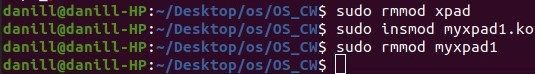
\includegraphics[scale=0.9]{img/sudo.jpg}
	\caption{Установка драйвера}
	\label{sudo}
\end{figure}\par

\subsection{Результат выполнения}
На Рисунке \ref{dmesg} показан вывод программы.
\begin{figure}[h!]
	\centering
	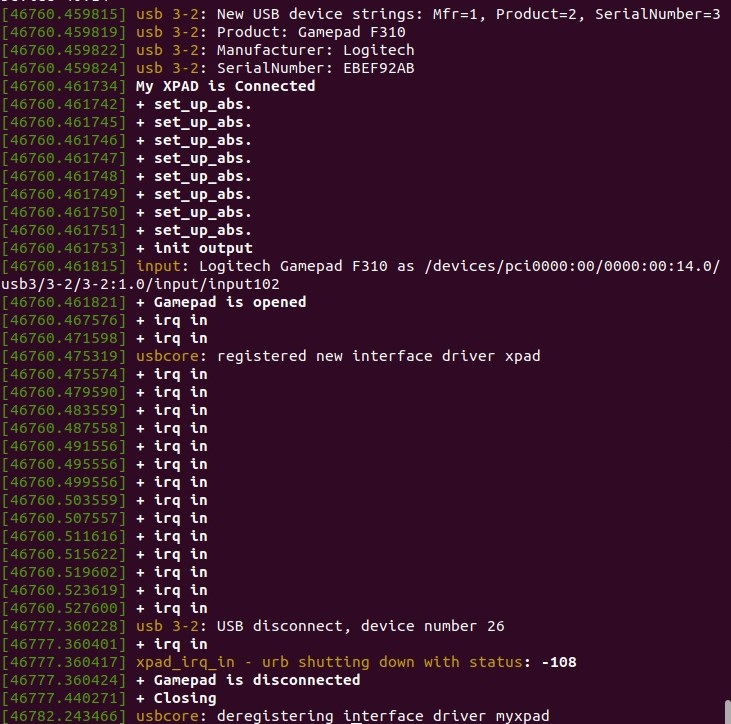
\includegraphics[scale=0.9]{img/ex1.jpg}
	\caption{Вывод программы}
	\label{dmesg}
\end{figure}\par





\pagebreak